%%%%%%%%%%%%%%%%%%%%%%%%%%%%%%%%%%%%%%%%%%%%%%%%%%%%%%%%%%%%%%%%%%%%%%%%%%%%%%%%
%2345678901234567890123456789012345678901234567890123456789012345678901234567890
%        1         2         3         4         5         6         7         8

\documentclass[letterpaper, 10 pt, conference]{ieeeconf}  % Comment this line out
                                                          % if you need a4paper
%\documentclass[a4paper, 10pt, conference]{ieeeconf}      % Use this line for a4
                                                          % paper

\IEEEoverridecommandlockouts                              % This command is only
                                                          % needed if you want to
                                                          % use the \thanks command
\overrideIEEEmargins
% See the \addtolength command later in the file to balance the column lengths
% on the last page of the document



% The following packages can be found on http:\\www.ctan.org
%\usepackage{graphics} % for pdf, bitmapped graphics files
%\usepackage{epsfig} % for postscript graphics files
%\usepackage{mathptmx} % assumes new font selection scheme installed
%\usepackage{times} % assumes new font selection scheme installed
%\usepackage{amsmath} % assumes amsmath package installed
%\usepackage{amssymb}  % assumes amsmath package installed

\usepackage[utf8]{inputenc}
\usepackage{graphicx}
\usepackage{endnotes}

\usepackage{mathtools}
\DeclarePairedDelimiter\ceil{\lceil}{\rceil}
\DeclarePairedDelimiter\floor{\lfloor}{\rfloor}

\usepackage{algorithm}
\usepackage{algpseudocode}
\usepackage{listings}
\usepackage{color}

\definecolor{miverde}{rgb}{0,0.6,0}
\definecolor{migris}{rgb}{0.5,0.5,0.5}
\definecolor{mimalva}{rgb}{0.58,0,0.82}

\lstset{ %
  backgroundcolor=\color{white},   % Indica el color de fondo; necesita que se añada \usepackage{color} o \usepackage{xcolor}
  basicstyle=\footnotesize,        % Fija el tamaño del tipo de letra utilizado para el código
  breakatwhitespace=false,         % Activarlo para que los saltos automáticos solo se apliquen en los espacios en blanco
  breaklines=true,                 % Activa el salto de línea automático
  captionpos=b,                    % Establece la posición de la leyenda del cuadro de código
  commentstyle=\color{miverde},    % Estilo de los comentarios
  deletekeywords={...},            % Si se quiere eliminar palabras clave del lenguaje
  escapeinside={\%*}{*)},          % Si quieres incorporar LaTeX dentro del propio código
  extendedchars=true,              % Permite utilizar caracteres extendidos no-ASCII; solo funciona para codificaciones de 8-bits; para UTF-8 no funciona. En xelatex necesita estar a true para que funcione.
  frame=single,	                   % Añade un marco al código
  keepspaces=true,                 % Mantiene los espacios en el texto. Es útil para mantener la indentación del código(puede necesitar columns=flexible).
  keywordstyle=\color{blue},       % estilo de las palabras clave
  language=Pascal,                 % El lenguaje del código
  otherkeywords={*,...},           % Si se quieren añadir otras palabras clave al lenguaje
  numbers=none,                    % Posición de los números de línea (none, left, right).
  numbersep=5pt,                   % Distancia de los números de línea al código
  numberstyle=\small\color{migris}, % Estilo para los números de línea
  rulecolor=\color{black},         % Si no se activa, el color del marco puede cambiar en los saltos de línea entre textos que sea de otro color, por ejemplo, los comentarios, que están en verde en este ejemplo
  showstringspaces=false,          % subraya solamente los espacios que estén en una cadena de esto
  stepnumber=2,                    % Muestra solamente los números de línea que corresponden a cada salto. En este caso: 1,3,5,...
  stringstyle=\color{mimalva},     % Estilo de las cadenas de texto
  tabsize=2,	                   % Establece el salto de las tabulaciones a 2 espacios
  title=\lstname                   % muestra el nombre de los ficheros incluidos al utilizar \lstinputlisting; también se puede utilizar en el parámetro caption
}

\title{\LARGE \bf
Tarea 1: Hadoop
}

%\author{ \parbox{3 in}{\centering Huibert Kwakernaak*
%         \thanks{*Use the $\backslash$thanks command to put information here}\\
%         Faculty of Electrical Engineering, Mathematics and Computer Science\\
%         University of Twente\\
%         7500 AE Enschede, The Netherlands\\
%         {\tt\small h.kwakernaak@autsubmit.com}}
%         \hspace*{ 0.5 in}
%         \parbox{3 in}{ \centering Pradeep Misra**
%         \thanks{**The footnote marks may be inserted manually}\\
%        Department of Electrical Engineering \\
%         Wright State University\\
%         Dayton, OH 45435, USA\\
%         {\tt\small pmisra@cs.wright.edu}}
%}

\author{Paula Navarrete, Sebastián Orellana}


\begin{document}



\maketitle
\thispagestyle{empty}
\pagestyle{empty}


%%%%%%%%%%%%%%%%%%%%%%%%%%%%%%%%%%%%%%%%%%%%%%%%%%%%%%%%%%%%%%%%%%%%%%%%%%%%%%%%

%%%%%%%%%%%%%%%%%%%%%%%%%%%%%%%%%%%%%%%%%%%%%%%%%%%%%%%%%%%%%%%%%%%%%%%%%%%%%%%%
\section{INTRODUCCIÓN}
Probando

\section{EXPERIMENTACIÓN}
\subsection{Interacción con Hadoop Distributed File System}
\begin{itemize}


    \item  Se escribió y leyó archivos de distinto tamaño, siendo crecientes en bloques de 10MB desde tamaño 10MB hasta 140MB, midiendo el tiempo de transferencia y de lectura. Se midió el tiempo de escritura analizando el archivo ``/var/log/hadoop-hdfs/hadoop-hdfs-namenode-localhost.localdomain.log" para la tarea put. El tamaño de bloque por defecto de hadoop es de 64BM, que es con el cual fueron escritos los archivos, contemplando así tamaños de archivo menores y mayores al tamaño de bloque.
    
    La figura \ref{fig:tpo_write} ilustra la evolución del tiempo de escritura según aumenta el tamaño de archivo.
    \begin{figure}
      \centering
        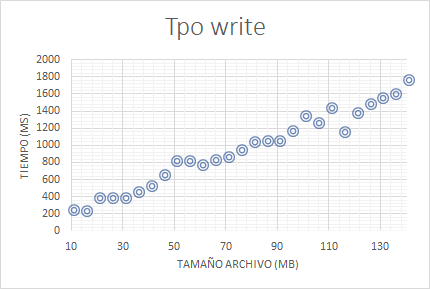
\includegraphics[width=0.5\textwidth]{tpo_write.png}
      \caption{Tiempo para escribir}
      \label{fig:tpo_write}
    \end{figure}
    
    En la figura \ref{fig:tpo_write} podemos apreciar que la velocidad de escritura no es lineal en el tiempo y tiende a disminuir a medida que el tamaño de archivo se acerca al tamaño de bloque, lo que explica la dismunución en el tiempo por cada MB copiado una vez que el archivo es levemente mayor que el tamaño de bloque. de aumento en el tiempo de transferencia es menor a medida que es cercana al tamaño de archivos.
    
    De igual manera, se midió el tiempo de lectura analizando el archivo ``/var/log/hadoop-hdfs/hadoop-hdfs-datanode-localhost.localdomain.log" al utilizar el comando cat para archivos crecientes en bloques de 10MB desde tamaño 10MB hasta 140MB, contemplando de igual forma tamaños de archivo menores y mayores al tamaño de bloque.
    La figura \ref{fig:tpo_read} ilustra la evolución del tiempo de lectura según aumenta el tamaño de archivo, pudiendo ver la misma tendencia que para el tiempo de escritura. 
    
    \begin{figure}
      \centering
        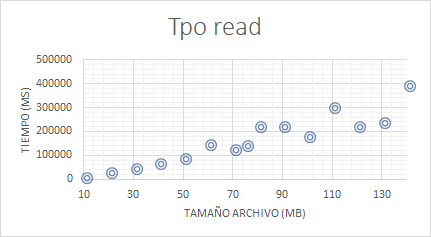
\includegraphics[width=0.5\textwidth]{tpo_read.png}
      \caption{Tiempo para leer}
      \label{fig:tpo_read}
    \end{figure}

    \item Se midió el tiempo de escritura analizando el archivo ``/var/log/hadoop-hdfs/hadoop-hdfs-namenode-localhost.localdomain.log" para la tarea put para archivos crecientes en bloques de 10MB desde tamaño 10MB hasta 110MB. El tamaño de bloque por utilizado al escribir los archivos en HDFS fue de 32 MB. 
    La figura \ref{fig:tpo_write_32mb_bs} ilustra la evolución del tiempo de escritura utilizando 32MB como tamaño de bloque según aumenta el tamaño de archivo.
    
    \begin{figure}
      \centering
        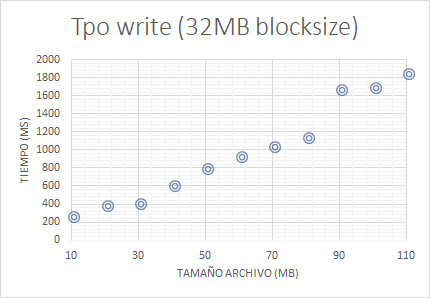
\includegraphics[width=0.5\textwidth]{tpo_write_32MB_blocksize.png}
      \caption{Tiempo para escribir (32MB tamaño bloque)}
      \label{fig:tpo_write_32mb_bs}
    \end{figure}

\end{itemize}

\subsection{Cuenta de Palabras}
A continuación, se emplea el paradigma de programación Map Reduce para contar la ocurrencia de cada una de las palabras que aparecen en un conjunto de documentos (\textit{word count}). La solución es implementada en Python, valiéndose para ello de la aplicación HadoopStreaming, que permite ejecutar funciones de Map y Reduce desde la \textit{shell} de la máquina virtual. 
\\

\noindent El código para la función Map es el siguiente:

\lstinputlisting[language=Python]{wordcount-mapper.py}

\noindent Y el código para la función Reduce:

\lstinputlisting[language=Python]{wordcount-reducer.py}

En particular, el conteo se realiza sobre el archivo \textit{palabras.txt}, guardando la salida en el archivo \textit{wordcount-output.txt} adjunto en la entrega. Notar que el delimitador entre palabras es exclusivamente el carácter espacio en blanco, lo cual implica que los pares de palabras del tipo \textit{(``virtual",``virtual.")} ó \textit{(``veces",``veces,")} sean contabilizadas con frecuencias independientes. Se decide no realizar ningún tratamiento adicional dadas las características del documento utilizado (texto extraído de una plantilla \LaTeX), que consta de palabras del tipo \textit{``\textbackslash{}texttt{A.key=B.Key}\textbackslash{}\textbackslash{}"}, que incluyen signos de puntuación y otros caracteres atípicos que de ser tratados podrían herir la semántica del texto. Situación similar se produce con el manejo de mayúsculas y minúsculas, donde a menudo diferencias en este aspecto se traducen en una amplia disimilitud en el espacio semántico subyacente. Así, de ser ignorado este comporatamiento, pares de palabras que incluyan siglas como \textit{(``siga",``SIGA")} ó \textit{(``un",``UN")} serían equivalentes, siendo que evidentemente representan distintos conceptos. No obstante, es factible realizar un tratamiento más agudo de este fenómeno que permita robustecer el conteo de palabras sin herir la semántica de los documentos, sin embargo se escapa del ámbito de esta actividad.

\subsection{Unión de datos: Parte 1}

En esta sección se implementa una aplicación típica de SQL: join. En particular se utiliza Hadoop para unir el contenido de los archivos \textit{dataCuentaTotal.txt} y \textit{dataCuentaDiaria.txt}. El archivo \textit{dataCuentaTotal.txt} contiene el resultado de la cuenta total de cierto grupo de palabras, empleando el formato $<$\textit{palabra,cuentaTotal}$>$. El archivos \textit{dataCuentaDiaria.txt} contiene el resultado de la cuenta diaria de palabras según fecha, utilizando el formato $<$\textit{fecha palabra,cuentaDiaria}$>$. El objetivo es unir (join) estos archivos, de tal manera que se genere un archivo de salida con la cuenta diaria y total de cada palabra, utilizando el formato $<$\textit{fecha palabra,cuentaDiaria cuentaTotal}$>$. 

Como una aplicación de este tipo podría servir para identificar fechas en las que determinadas palabras aparecen más de lo usual, la salida se ordena por defecto en función de las palabras. Luego, como también podría servir para identicar palabras que en determinadas fechas aparecen más de lo usual, la salida se puede ordenar (alfabéticamente por medio del flag \textit{-D mapred.text.key.comparator.options = '-k1,1}) en función del campo fecha. Ambos archivos de salida se adjuntan a la entrega, con nombres \textit{join-output.txt} y \textit{join-output-fecha.txt} respectivamente.  
\\

\noindent El código en Python para la función Map es el siguiente:

\lstinputlisting[language=Python]{join-mapper.py}

\noindent Notar que una elección apropiada de \textit{key} por parte del mapper corresponde  al campo en común de ambos archivos: \textit{palabra} (sobre el cual se quiere combinar los datos). Luego, (\textit{fecha}, \textit{cuentaDiaria}, \textit{cuentaTotal}) corresponde al \textit{value} de cada palabra. El código Python para la función Reduce es:

\lstinputlisting[language=Python]{join-reducer.py}

\noindent Así, teniendo en cuenta que el mapper deja los datos ordenados por \textit{key}, al reducer le basta con recorrerlos secuencialmente para identificar el último par (\textit{key,value}) por palabra, asignar la \textit{cuentaTotal} respectiva e imprimir la salida. 

\subsection{Unión de datos: Parte 2}
Por último, se repite la unión de documentos efectuada en la sección anterior, pero en este caso sobre dos tipos de archivos: \textit{i)} Información de programas de televisión que son emitidos por distintos canales, e \textit{ii)} Información del número de televidentes que observan distintas emisiones de cada programa. El objetivo es implementar funciones de Map y Reduce que permitan calcular el total de televidentes que ve cada uno de los programas emitidos por cierto canal de televisión. El código en Python para la función Map es el siguiente:

\lstinputlisting[language=Python]{join2-mapper.py}

\noindent Nuevamente la elección apropiada de \textit{key} por parte del mapper corresponde  al campo en común de ambos archivos: \textit{programa}. Notar que el mapper maneja la posibilidad de que cada combinación (\textit{TvShow, channel}) pueda aparecer múltiples veces, seteando por defecto el campo \textit{audiencia} en cero, por lo que repeticiones de registros no interfieren en la suma de total de audiencia.  

El código Python para la función Reduce es:

\lstinputlisting[language=Python]{join2-reducer.py}

\noindent Así, teniendo en cuenta que el mapper deja los datos ordenados por \textit{key}, al reducer le basta con recorrerlos secuencialmente para identificar el último par (\textit{key,value}) por programa, y asignar la suma total de audiencia asociada a las múltiples combinaciones (\textit{TvShow, audiencia}).

Notar además, que para este caso particular el reporte obtenido corresponde a la cuenta de los televidentes que vió programas de CAB (archivo de salida \textit{join2-output.txt} adjunto en la entrega), lo cual es filtrado directamente en el mapper con el fin de manejar circunstancias en que un mismo programa de televisión es emitido por varios canales. Para cambiar el canal bajo análisis basta con modificar el valor que se asigna a la variable \textit{canal} en la línea 21 del código del mapper.  

\section{CONCLUSIONES}

De la interacción con l sistema de archivos



HDFS almacena archivos en el clúster dividiéndolos en bloques de tamaño fijo siendo el 64MB el tamaño de bloque HDFS predeterminado en Hadoop. El tamaño de bloque puede afectar el rendimiento de las operaciones del sistema de archivos donde los tamaños de bloque más grandes serían más efectivos si está almacenando y procesando archivos muy grandes. El tamaño de bloque de datos también puede afectar el rendimiento de los cálculos de MapReduce, ya que el comportamiento predeterminado de Hadoop es crear una tarea map para cada bloque de datos de los archivos de entrada.


\addtolength{\textheight}{-12cm}   % This command serves to balance the column lengths
                                  % on the last page of the document manually. It shortens
                                  % the textheight of the last page by a suitable amount.
                                  % This command does not take effect until the next page
                                  % so it should come on the page before the last. Make
                                  % sure that you do not shorten the textheight too much.


\begin{thebibliography}{99}

\bibitem{c1} 





\end{thebibliography}




\end{document}
